\documentclass[onecolumn,nocopyrightspace,preprint]{sigplanconf}

\usepackage{booktabs}
\usepackage{listings}
\usepackage{hyperref}
\usepackage{xspace}
\usepackage{caption}
\usepackage[tocentry]{vhistory}
\usepackage{graphicx}
\usepackage{natbib}
\usepackage[utf8]{inputenc}

% \lstset{
%   commentstyle=\small\ttfamily, %
%   fontadjust=true, %
%   firstnum  ber=1, %
%   escapeinside={(*}{*)}, %
% }

\lstset{
  float=*,
  numbers=none,
  numberstyle=\footnotesize,
  numbersep=4pt,
  basicstyle=\small\ttfamily,
  keywordstyle=\small\ttfamily\bf,
  tabsize=2,
  breaklines=true,
  frame=lines,
  aboveskip=\bigskipamount,
  belowskip=\bigskipamount,
  %belowcaptionskip=\medskipamount,
  language=bash,
  deletekeywords={env, for}
}

\nocaptionrule



\title{Antescofo: The Artificial Musician}
\authorinfo{
  Martin~Aigner
}{Computational Systems Group\\University of Salzburg}{firstname.lastname@cs.uni-salzburg.at}

\begin{document}
\maketitle
%\tableofcontents


%First, introduce project and how to create motivation to learn.
%Second, derive objectives and tasks
%Third, cover material to enable learning what it takes to achieve the objectives
%Finally, wrap up, and thats it


\section{Foreword}  

Writing this report is part of the requirements of the course ``Software Usage
in School: An Overview'' intended to make participants think about combining
different teaching topics through a single common property: the use of
computers.

The goal is to propose a hypothetical interdisciplinary project using at least
three different software tools. The cool thing here: this project has actually
happened. The drawback: it is no longer a hypothetical project and therefore,
kind of, contradicts the task of thinking about: ``How would I plan and lead
that project?'' Nevertheless, we did plan the project in advance as much as
possible and clearly state any changes we have applied  to \textit{the plan}
during the project. Still, we have improvised a lot, e.g., making up on-demand
mini lectures on the fly. The interested reader might wonder if improvisation
further contradicts the idea of planning and describing a hypothetical
project.  We don't think so! A teachers ability to adapt to individual
student's knowledge, needs, and interests is, in our opinion, a key quality to
have in the educational business.

With this report, want to enable others to repeat the project under similar
circumstances. The goal of the project itself is to enable students to perform
similar tasks in the future on their own.  The students achieved a great
result which can be watched at \url{https://youtu.be/a_AVsBpvBVo}

\section{Background of the Project aka. the Original Plan}\label{sec:background}

The Computational Systems Group Salzburg is involved in a research project on
Antescofo, a real-time multimedia system, developed by IRCAM, Paris. Antescofo
is a complex piece of software used to accompany musicians and orchestras on
the stage. It is used at various concert halls throughout the world, including
the Festspielhaus in Salzburg. We have recently submitted a research proposal
with IRCAM on advancing the real-time aspects of Antescofo for embedded
devices. From that proposal we derived the idea of a student internship
project.

The task of the students within this internship is to setup, use, and thereby
do a performance analysis of Antescofo. Some of the challenges of Antescofo
are scalability, as well as proper modeling of time, topics that our research
group has expertise on. The students are expected to get Antescofo running in
a lab environment, demonstrate simple use with an actual instrument, and
isolate performance issues that motivate our research. This internship
project will be a valuable kick-off for our research on enhancing the 
real-time aspects of Antescofo.

Assets for the students are to experience working on a highly sophisticated
software system, getting acquainted with technical issues of setting up a
system, and experience with research on real-time aspects of computing. The
ultimate goal: having fun with music and complex software.


\section{An Interdisciplinary Project}

The goal of this report is to describe an interdisciplinary project and
introduce software that aids the education in each discipline.  We believe
that, in fact, every project is interdisciplinary in one way or another, even
if it is not obvious on first sight. In our case, however, it is very easy to
map certain parts of the project to three school subjects. First of all we
have computer science. Working with Antescofo requires programming a computer.
The students even have to learn a distinct programming language, called Pure
Data. Secondly, there is music education. The students need to understand what
they write in their programs so reading and writing a musical score is a
requirement for this project. Thirdly and finally we have media art. We want
to present the result of project, a piece of music, to an audience and since
\textit{video killed the radio star} we produce a music video.
Section~\ref{sec:material} gives an overview of the tools. There was, in fact,
more software involved in the final result but we skip detailed descriptions
of those tools for brevity.


\subsection{Motivation of the Students}

For a successful project each team member should participate with about the
same amount of passion and interest.  The high level goal of the project is
simple, yet challenging: Making music with computers. To raise the students
interest and motivation we try to connect the topics of the project with prior
experience and expertise of the students.

The initial goal of the project was evaluating real-time constraints of
Antescofo. However, in an early stage of preparing the project it became clear
that this goal was way too challenging for high-school students without the
required background in real-time systems. Therefore, we changed the scope from
a technical evaluation of the software to an exploration of its artistic
capabilities. We set a new objective: Having fun in the creative process of
making music with computers.

During the first days of the project we did a number of informal conversations
about the things we were going to do, taking notice of student's interests in
certain aspects and student's knowledge that might aid the project. We discussed
similar projects and how they were realized. We sketched rough plans for similar
projects and let the students guess any requirements so that they understand
the importance of acquiring new skills in order to realize the new tasks. We
took notice of the students motives behind attending the project to eventually
empower them in achieving their own goals. Making the students curious about the
project and the related tasks facilitates their own motivation in learning the
required material.

It is important to motivate the students to spend a lot of time learning to
handle a complex piece of software. Antescofo is designed to be used by
professionals in either (or both) computer science and composition. The
technical documentation of Antescofo is hard to read and understand for non
computer scientists and therefore it is important to make the students
understand that it is possible to achieve the project goal. Fortunately, there
exist a number of examples of the application of Antescofo in an artistic
context on youtube. The students realized that the project was doable from the
beginning. The final result of the project was the ultimate confirmation.

\subsection{Take four teenagers and make them a Team}\label{sec:team}

This project is a group project. So the first thing we need to successfully
realize that project is making a team out of four students from different
educational backgrounds. Usually, in the context of a class room, the students
already know each other and, in the best case, teachers know the students as
well. In our project, this was not the case. The students did not know each
other beforehand and the instructor did not know them either so we had to
spend some time on getting the initial shyness out of the way.
In such a case it is necessary to getting to know each other up to a level
where communicating about project related topics is no longer negatively
effected by personal insecurities. The instructor is responsible for setting
up a safe environment where thoughts can be shared without judgment and
stereotypes related to the students background, gender, personal interests, etc.

We managed to build an effective Team with 4 students from three different
schools.  It should be even simpler with students from the same school or even
the same class. Still, as we shall learn from actually doing the project, we
could exploit the differences among the students by assigning different tasks
according to individual strengths and interests. A challenging but rewarding
effort!

We started by having the students introduce themselves, effectively becoming
part of the group. They had to answer to four questions: What's your name?
Tell us about your school?  What would you like to learn in this project?
Anything you like to do besides music, like, hobbies? Note that the instructor
answered to the same questions as well.  We planned to take particular
interest in the answers to question 3. However, the students could not really
come up with specific things they wanted to take out of the project. This led
us to the conclusion that the initial description of the project's objectives
was either too technical, too abstract, or simply not interesting enough.
However, after the project was finished, we gladly realized that boredom was
not the case. While writing this report, we figure that we should have asked
the students for their reasons to not having any specific questions in the
beginning.

After the initial introduction and a more detailed description of the project
objectives, we left the students on their own to discuss any ideas they might
have in mind. We asked them to discuss, if they wanted to, their musical
socialization, what they like to listen to, how they did come to playing and
making music, and so on. The result of the student's brainstorming session
was included in our project goals described in Section~\ref{sec:objectives}.
The interested reader will notice quite significant changes to the initial
project goals highlighted in Section~\ref{sec:background}.


\subsection{Environment}

Enabling the students to learn on their own requires putting them in the
proper environment. Building a group creates a social environment but it is
also important to create the right spacial environment. For this project the
requirements for the teaching and learning space are obvious. We need to be
able to listen to and play music without disturbing others. We need basic
equipment for recording music and for shooting video scenes. We need computers
running the required software and  Internet access for research purposes. In
other words: we need a studio. So we built one! We exclusively reserved a
seminar room and provided very basic, yet functioning audio and video
equipment, i.e., a mixing console, microphones, a video camera, Apple laptops
(may be adapted when using different software products). The students provided
their own instruments.


\section{Project Details}\label{sec:objectives}

This section describes the objectives of the project and the material we
provide for the students to acquire the required skills. The students learn by
example and finding their own answers to specific tasks and questions.

\subsection{Objectives}

During the preparation phase of the project we noticed that running Antescofo
and incorporating the software in a piece of music is quite a challenging task
on it's own. We therefore decided to adapt the project objectives of our initial
project idea such that we will achieve a satisfactory result within the limited time
frame of the project. We decided to keep the performance and real-time analysis of
Antescofo as an optional project extension after we finished the primary goal:
\textit{by the end of the project the students are enabled to employ software
tools in the creative process of making music.}

From the high level objective, we can derive a list of skills the students
have to acquire in order to implement such a project.

\begin{description} 

\item[Playing music:] The students were already trained in playing different
instruments. We decided to adapt the project to that existing skill set, if
necessary.

\item[Getting music in the computer:] The students need to know basics of the
different types of I/O in the context of digital music production, e.g., audio
streams, control sequences, analog-to-digital conversion (ADC).

\item[The physics of sound:] Getting music in the computer requires capturing
sounds in the first place. The students need to learn what sound is, the basics
of acoustic instruments, microphones, and amplifiers, e.g., dynamic range,
headroom, distortion, the role of noise.

\item[Synthetic instruments:] Interested students will learn the basics of the
synthesis of sound, i.e., waveform generation, filters, relationship of the
frequency spectrum and tone.

\item[Programming Antescofo:] Antescofo is based on Pure Data. The students
have to learn the basics of this programming language and also the syntax of
the musical notation in Antescofo.

\item[Working with an analog mixing console:] The students will learn to
identify the different stages of amplification and mixing on a mixing console.

\item[Working with a digital audio workstation:] The students will learn
connecting different musical software tools through standardized software
interfaces, e.g., MIDI signals or Apple's inter-application communication
(IAC) drivers. The students will understand the similarities and differences
in routing audio and control messages in hardware and software.

\item[Making a music video:] This objective we keep vague, by design. It
depends on the actual piece, the actual instruments, and the attitude of the
students. We noticed that not every student is willing or capable to perform
in front of a camera. The students, however, will learn to combine separate
video and audio tracks in one final piece that presents all skills acquired
during this project.

\end{description}

One last objective remains: the piece of music that will be performed in the
end. This objective is set by the students. In our case the students wanted to
perform the song ``Bad Romance'' by Lady Gaga. This was not planned in
advance, but emerged while the initial playing phase with Antescofo. The
students decided to have a singer as soloist and the singer chose that song
because of prior experience with the material.


\subsection{Course Material}\label{sec:material}


This section lists the material that aids learning the required skills listed above.

\begin{description}

\item[Playing music:] We provide a lead sheet of ``Bad Romance''. The teacher
makes sure that the students understand the song structure and the cord progression
to make the computer accompany the song. 

\item[Getting music in the computer:] We provide a short lecture on the basics
of analog-to-digital conversion (ADC). We discuss advantages and disadvantages
on a conceptual language. It is not necessary to know implementation details
of ADCs but it is important to understand where and why it is applied in the
signal processing chain.

\item[The physics of sound:] We keep this topic very basic. Understanding the
relation between frequency and pitch, amplitude and volume, and the sum of
frequencies and tone is essential but sufficient for this project. Related
Wikipedia sources and a short lecture on the physics of audio resemble the
material for this task.

\item[Synthetic instruments:] From the physical analysis of sound we directly
derive the synthesis of sound. Once the students understand that sound is a
sum of different frequencies  with different amplitudes they understand that
one can generate sound by mixing different frequencies with different
amplitudes which is the very concept of a synthesizer. We provide a short
lecture on analog synthesizers covering the basic principles. Then we
provide a set of software synthesizers to the students to play with. By
changing certain parameters of the synthesis they can immediately hear the
result and thereby connect the abstract idea of shaping sound with the
concrete sound in their ears. Pure Data (see below) also provides help patches
illustrating the internals of synthesizers.

\item[Programming Antescofo:] Antescofo is implemented in Pure Data. To
interact with Antescofo, the students need to learn basics of Pure Data first.

``Pure Data (aka Pd) is an open source visual programming language. Pd enables
musicians, visual artists, performers, researchers, and developers to create
software graphically, without writing lines of code. Pd is used to process
and generate sound, video, 2D/3D graphics, and interface sensors, input
devices, and MIDI. Pd can easily work over local and remote networks to
integrate wearable technology, motor systems, lighting rigs, and other
equipment. Pd is suitable for learning basic multimedia processing and
visual programming methods as well as for realizing complex systems for
large-scale projects.''~\cite{website:puredata}

\begin{figure}[t]
    \centering
    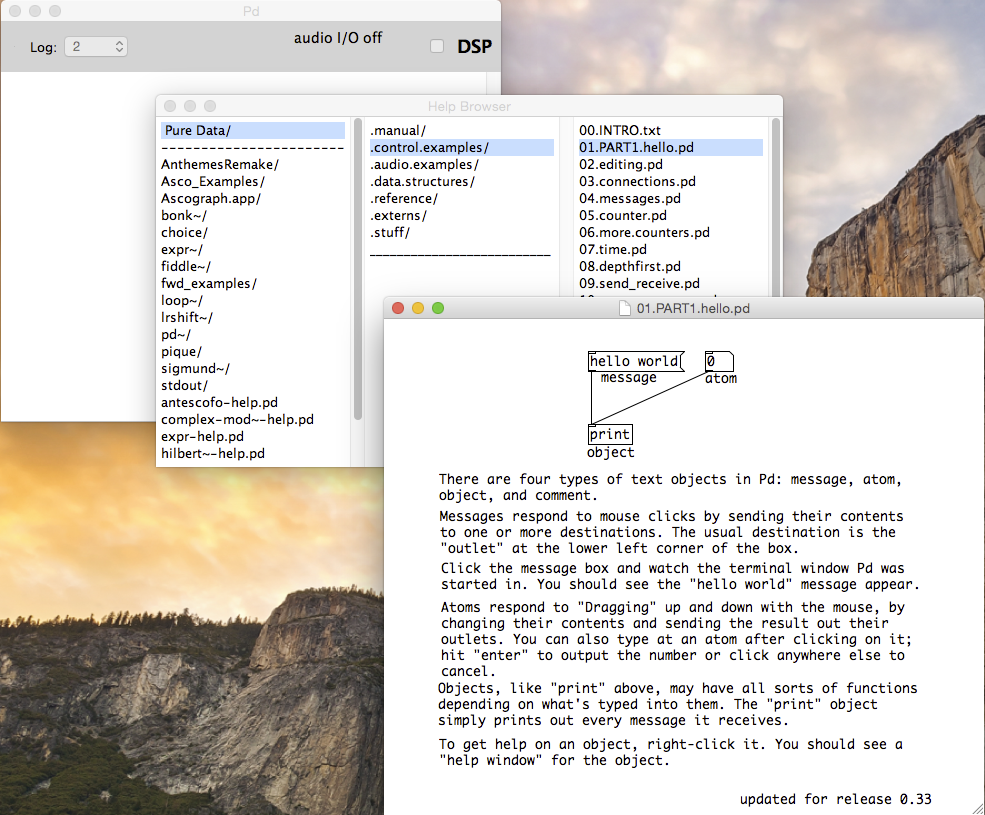
\includegraphics[scale=0.4]{fig/pd-help-browser.png}
    \caption{Pure Data Help Browser}
    \label{fig:pd-help-browser}
\end{figure}

We point the students to the online help browser of Pure Data, illustrated in
Figure~\ref{fig:pd-help-browser}, and demonstrate its application. The help
browser is made up of Pure Data programs, called patches, that allow immediate
interaction with the programming examples.

``Antescofo is a modular polyphonic Score Following system as well as a
Synchronous Programming language for musical composition. The module allows
for automatic recognition of music score position and tempo from a realtime
audio Stream coming from performer(s), making it possible to synchronize an
instrumental performance with computer realized elements. The synchronous
language within Antescofo allows flexible writing of time and interaction in
computer music.''~\cite{website:antescofo}

\begin{figure}[ht]
    \centering
    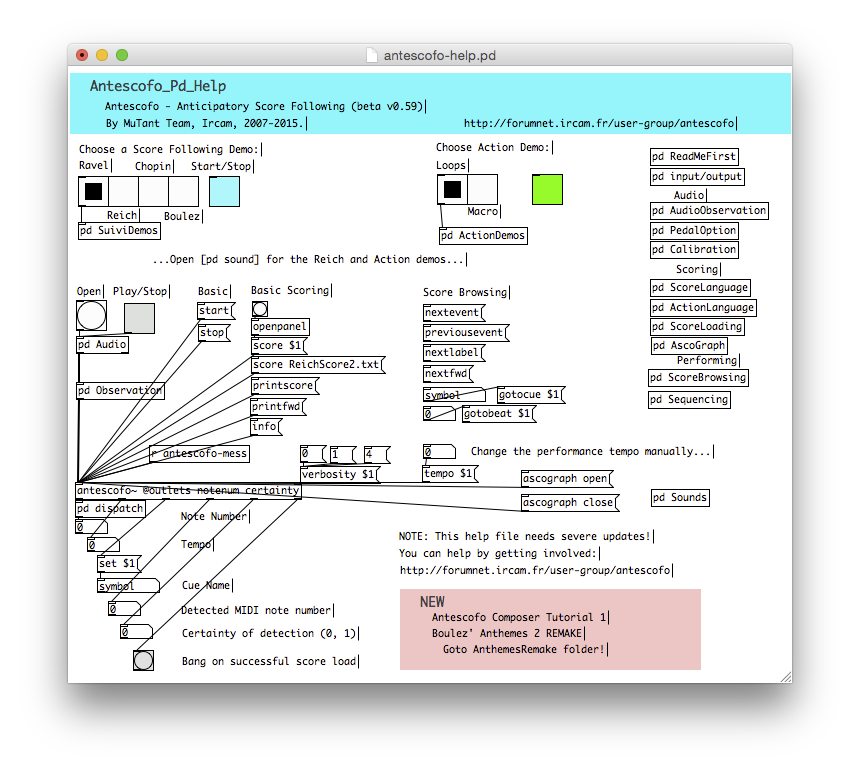
\includegraphics[scale=0.5]{fig/ascohelp.png}
    \caption{Antescofo Help Patch}
    \label{fig:ascohelp}
\end{figure}

Additional material we provide include the official technical documentation,
demo patches prepared by the instructor, asking questions in the Antescofo
user group, and backward-engineering under supervision, i.e., students take a
look at the Antescofo demo programs as shown in Figure~\ref{fig:ascohelp} and
explain what they discover to the teacher.


\item[Working with an analog mixing console:] We provide a simple 12-track
analog Mixing console and its manual. Based on its block schematic we
explain the signal flow inside a mixer and point the students to application
examples in the manual. The students need to find out which of the application
examples fits the requirement of the project and how to set up the console
accordingly under supervision. Unfortunately, copyright limitations do not
allow for inclusion of the block schematics in this report. See the website of
any manufacturer of mixing consoles, e.g., mackie.com, for manuals, use cases,
and applications.

\item[Working with a digital audio workstation:] For acquiring this skill it
is important to understand analog mixing and routing first because most
digital audio workstations emulate hardware consoles in look and feel. Once
the students find themselves familiar with a hardware mixer and recording
equipment, they will have no issues repeating the same steps in software. For
our project, we use Logic Pro~\cite{website:logic}, which is a professional
MIDI and audio recoding software for OSX. It supports all features required
for the project, i.e., processing multiple audio tracks together with real-
time MIDI instruments for synthesizing sounds while playing with Antescofo and
recording the piece in high quality.  Note that there are many similar tools,
including free and open source software, that would do the trick.
Nevertheless, we choose Logic Pro for one reason. One of the students had
prior knowledge with Logic Pro. Additional material we provide include
examples of multi-track multi- instrument projects showing the non-linear
production process of software sequencers. Once the students learn the work
flow of multi-track audio production, all tools suddenly look similar.

\item[Making a music video:] Similar to the choice of Logic Pro, there are
plenty of alternative software tools to do the job. Again, one student had
prior knowledge in working with iMovie.

``iMovie is a video editing software application sold by Apple Inc. for the Mac
and iOS. It was originally released in 1999. ... From 2003, iMovie is included
free with all new Mac computers. iMovie imports video footage to the Mac using
either the FireWire interface on most MiniDV format digital video cameras or
the computer's USB port. It can also import video and photo files from a hard
drive. From there, the user can edit the photos and video clips and add
titles, themes, music, and effects, including basic color correction and video
enhancement tools and transitions such as fades and slides. There are
currently hundreds of iMovie video tutorials online.''~\cite{website:imovie}

The students prior knowledge was sufficient to achieve simple results with
iMovie. Only few questions had to be covered by the instructor.

\end{description}




\section{Time Table}

The students spent 4 weeks at our department. During the first week all students
got a lecture on computer science basics not covering any project-specific topics yet.

The time frame for the project itself was approximately 3 weeks, 6 hours per day.
Note that the time table is heavily affected by the students' prior
knowledge in programming. Table~\ref{tab:time} gives a brief overview of the
suggested time required for each individual project task.

\begin{table}
\centering
\begin{tabular}{l|ll}
When              & What  & How  \\
\hline
Week 1            & Teambuilding          & see Section~\ref{sec:team} \\
                  & The physics of sound  & see Section~\ref{sec:material} \\
                  & Synthetic instruments & see Section~\ref{sec:material} \\
                  & Environmental setup   & prepare computers, software, hardware and develop intuition by 
                  \\
                  &  & playing with it (performed in parallel to other tasks)  \\
Week 2            & Pure Data             & building first patches,see Section~\ref{sec:material} \\
                  & Synthetic instruments cont. & audio synthesis in Pure Data \\
                  & Playing Music   & preparing and practicing ``Bad Romance'' \\
                  & Antescofo & building a simple working Antescofo demo \\
Week 3            & Antescofo cont. & implementing ``Bad Romance'' in Antescofo \\
                  & Synthetic instruments cont.  & controlling instruments through MIDI \\
                  & Performance   & Rehearse and record audio and video of ``Bad Romance'' \\
                  & Production   & combine media in the final music video \\
\end{tabular}
\caption{Timetable}
\label{tab:time}
\end{table}

\subsection{Teaching style}

For this project we mixed different teaching styles. Group based work,
individual training, lecture based classes, and a democratic decision
process.~\cite{book:Hubwieser2007} We did short lectures and then let the
students experiment with the topics of the lecture. Most of the time the
students worked on their own, interrupted by progress reports twice a day.
There they could elaborate issues and the teacher could guide them in finding
answers. They were allowed to try their own ideas in the environment of a
studio to see what works and to make mistakes to see what does work. The
environment was designed to be fault tolerant.

We want to enable the students to find their own answers in the materials we
provide. Therefore, selecting the material is done with one thought in mind:
``Does the material fit the students?'' This is hard to tell in advance so we
observed the way the students interacted with the material. In case there were
problems we would change the selection of material or help the students to
overcome problems with the material. We also encouraged the students to find
their own material: ``Did you google it?'' The students then explained their
findings to the instructor and applied their new knowledge under supervision.

Any artistic choices were left to the students because we wanted to have the
students find their own aesthetic expressions.~\cite{book:Peez2008}

\section{Conclusion}

We had great fun realizing this project. It was the first time for the high-
school students working at a university and it was the first time for the
instructor teaching high-school students. We conclude that adapting the
initial project objectives to a simpler task that had a higher chance of
success was a good decision because the students got challenging tasks and
still the impression  that the goals are achievable. That kept the motivation
high throughout the project and enabled all participants to successfully
finish their goals.

\section{Acknowledgments}

The project was supported by the Austrian Research Promotion Agency (FFG) FFG-
Nr 851846, but it was only possible because of the students: Matthäus Mayr,
Amrita Newton, Hannah Schmidbauer, and Leonard Trommler. Thanks a lot!

\bibliographystyle{IEEEtran}
\bibliography{sources} 


\end{document}


